
These appendices contain examples of common use cases that hopefully might prove useful as reference material, especially for those new to LaTeX.
Assuming you're working in the editor of overleaf.com, the markup for all the examples below can be found by clicking on \verb|example_appendix.tex| under the \verb|Appendices| folder in the left hand project overview.


% =-=-=-=-=-=-=-=-=-=-=-=-=-=-=-=-=-=-=-=
% REFERENCES
% =-=-=-=-=-=-=-=-=-=-=-=-=-=-=-=-=-=-=-=
\subsection{References}


When writing, you often have to refer back to something you said earlier, forward to something you will get back to later, to figures and tables, or to external sources.

\subsubsection{Within the Document}
\label{app:within-the-document}

Sections, figures, tables, and pretty much anything in a latex document can be labeled and cross-referenced.
For instance, this (subsub)section is labeled with \verb|\label{app:within-the-document}|, allowing it to be referenced throughout the document.
The advantage of labeling and referencing is that it allows the correct element code (A1 at the time of writing) to be generated at compile time, which in turn reduces the chance that old references become outdated as the project evolves over time.

After an element is labeled, it can be referenced in several ways:

\begin{itemize}
    \item Reference element code: \verb|\ref{app:within-the-document}| $\rightarrow$ \ref{app:within-the-document}
    \item Reference element page \verb|\pageref{app:within-the-document}| $\rightarrow$ \pageref{app:within-the-document}
    \item Autoformat reference\footnote{The exact format of autoref is configurable. See "setup.sty".}: \verb|\autoref{app:within-the-document}| $\rightarrow$ \autoref{app:within-the-document}
\end{itemize}

\subsubsection{Citations}

Referencing to external work, in the form of citations, requires two steps.
First, descriptions of the relevant work must be made available.
In this project, the content of "references.bib" will be taken into account when compiling the project.
This file can be populated manually, which is fine for smaller projects with only a handful of citations.
Alternatively, if you're using a reference manager such as Zotero or Mendeley to organize your collection of pdfs, they typically come with a function to export a .bib file that can be uploaded to the project.
However, the process can be further streamlined by connecting your reference manager directly to overleaf (see \url{https://www.overleaf.com/blog/639-tip-of-the-week-overleaf-and-reference-managers}).

Once the bibliography is made available, it can be cited:

\begin{itemize}
    \item \verb|\cite{ghia_et_al}| $\rightarrow$ \cite{ghia_et_al}
    \item \verb|\citep{ghia_et_al}| $\rightarrow$ \citep{ghia_et_al}
    \item \verb|\citep{ghia_et_al, sagan_1993}| $\rightarrow$ \citep{ghia_et_al, sagan_1993}
\end{itemize}

Cited bibliography will automatically show up in the bibliography section of this document.
The exact appearance depends on the configured citation style, which at the time of writing is set to \verb|plainnat| (see \url{https://www.overleaf.com/learn/latex/Natbib_bibliography_styles} for alternatives).

% =-=-=-=-=-=-=-=-=-=-=-=-=-=-=-=-=-=-=-=
% FIGURES
% =-=-=-=-=-=-=-=-=-=-=-=-=-=-=-=-=-=-=-=

\subsection{Figures}

Beautiful figures will make your report pop. The subsequent examples cover some of the most common ways to insert them into the document.

\subsubsection{Simple Figures}

Figures are declared with the \verb|\being{figure}...\end{figure}| command.
You can put different forms of graphics inside it, but the most common use case involves loading graphics from an external image file.
Similarly to sections, images can be labeled and referenced throughout the document (see Figure \ref{fig:example-figure}).

\textbf{Note:} If you did not produce the figure content yourself, remember to credit the original author.


\begin{figure}[H]  % Place figure (H)ere. I.e. don't float it around 
    % Center figure 
    \centering
    % Display image
    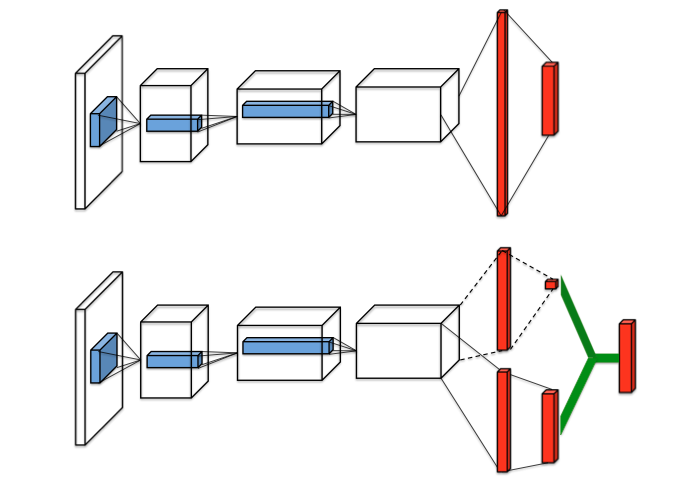
\includegraphics[width=0.5\textwidth]{Images/example_figure.png}
    % Add caption, label, and source 
    \caption{Example figure}
    \label{fig:example-figure}
    \source{\cite{DBLP:journals/corr/WangFL15}}
\end{figure}


\subsubsection{Sub-figures}

It is also possible to compose a single figure from several graphical elements.
Figure \ref{fig:example-sub-figure} gives an example of how this can be done with the use of subfigures.

% Declare outer figure 
\begin{figure}[H]
    \centering
    % Place each image in it's own sub-figure 
    \begin{subfigure}[t]{0.450\textwidth}
        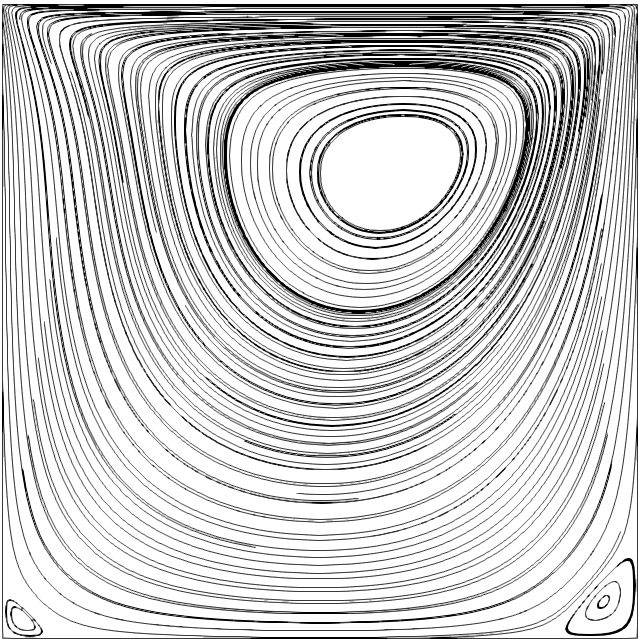
\includegraphics[width=\textwidth]{Images/Sub-figures_Example/cavity_100_streamlines.png}
        % Caption specific for sub-figure
        \caption*{$Re = 100$ - Testing method.}
    \end{subfigure}
    % Repeat for new sub-figure
    \begin{subfigure}[t]{0.441\textwidth}
        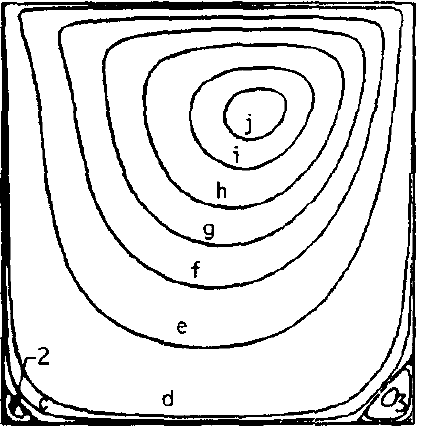
\includegraphics[width=\textwidth]{Images/Sub-figures_Example/cavity_100_streamlines_ghia.png}
        \caption*{$Re = 100$ - \citet{ghia_et_al}.}
    \end{subfigure}
    % Add caption and label for overall figure 
    \caption{Example sub-figures}
    \label{fig:example-sub-figure}
\end{figure}


\subsubsection{Generated Diagrams}

There are also several packages for generating figures and diagrams.
Figure \ref{fig:example-flow-chart} was generated with the \verb|tikz| package, which allows drawing arbitrary vector graphics with LaTeX commands.
While elegant, learning it might take some time, so an easier solution is to use conventional drawing tools with graphical user interfaces (e.g. \url{draw.io}) and display the resulting figures as conventional images.

\begin{figure}[H]
    \centering
    % Draw figure using tikzpicture commands 
    \begin{tikzpicture}[node distance = 2cm, auto]
        % Place nodes
        \node [block] (init) {Learning \LaTeX};
        \node [cloud, left of=init] (you) {You};
        \node [block, below of=init] (new_project) {Making new project};
        \node [decision, below of=new_project] (decide) {Good enough?};
        \node [block, right of=new_project, node distance=3cm] (no) {Improve the template};
        \node [block, below of=decide, node distance=3cm] (yes) {Get to work!};

        % Draw edges
        \path [line] (init) -- (new_project);
        \path [line] (new_project) -- (decide);
        \path [line] (decide) -- node {Yes} (yes);
        \path [line] (decide) -| node [near start] {No} (no);
        \path [line] (no) -- (new_project);
        \path [line,dashed] (you) -- (init);
    \end{tikzpicture}
    \caption{Example of generated flow chart}
    \label{fig:example-flow-chart}
\end{figure}


% =-=-=-=-=-=-=-=-=-=-=-=-=-=-=-=-=-=-=-=
% TABLES 
% =-=-=-=-=-=-=-=-=-=-=-=-=-=-=-=-=-=-=-=
\subsection{Tables}
\label{app:tables}

Similarly to other markup languages, such as HTML, LaTeX documents are fundamentally one-dimensional, making two-dimensional concepts, such as tables, somewhat annoying to deal with. The following examples document ways to create and manage tables in LaTeX projects.

\subsubsection{Basic}

In the simplest case, tables can be created by manually typing out a set of LaTeX commands enclosed in a set of \verb|\begin{table}...\end{table}| tags.
Similarly to figures and sections, they can also be labeled and cross-referenced throughout the documents (see source for Table \ref{tab:example-table} for a commented example).
Getting the formatting right can be a bit cumbersome, but there exists serveral websites\footnote{Latex table generator: \url{https://www.tablesgenerator.com}} that can be used to generate the necessary markup from a simpler user interface.

% Initialize table. "!h" prevents the it from floating around
% See: https://www.overleaf.com/learn/latex/Errors/%60!h'%20float%20specifier%20changed%20to%20%60!ht'
\begin{table}[H]
    % Place the table in the center of the page 
    \centering
    % Define 3 columns: 1 (l)eft-aligned, then a horizontal line, then two (c)enter-aligned
    \begin{tabular}{l|cc}
        % Put a thick line on top the table and add header row
        \toprule
        Statistic & Agent57 & R2D2 (bandit) \\
        % Separate header by a slimmer line and add body
        \midrule
        Mean      & 4766.25 & 5461.66       \\
        Median    & 1933.49 & 2357.92       \\
        % Put a thick line at the bottom 
        \bottomrule
    \end{tabular}
    % Add a caption with text that will appear below the table
    \caption{This is an example table.}
    % Add a label so the table can be referenced with \ref{...}
    \label{tab:example-table}
\end{table}

\subsubsection{Using Python}

Alternatively, if the data you wish to visualize is already in python, the pandas package can be used to generate LaTeX markup as a string that can be copied into the LaTeX document.

\usemintedstyle{default}
\begin{minted}{python}
import pandas as pd 
df = pd.DataFrame(table_data)
# Generates a latex table
tex1 = df.to_latex()
# Generates a latex table without the DataFrame's index as a column
tex2 = df.to_latex(index=False)
# Alternatively, save it to csv and use the method in the next section
df.to_csv('table_data.csv')
\end{minted}

Note that the \verb|to_latex| method will by default only generate the \verb|\begin{tabular}...\end{tabular}| part of of the table. Additionally, sometimes it may not generate the exact format you might be looking for. However, a lot of this can be fixed with optional key-word arguments that are further explained in the pandas documentation (see  \url{https://pandas.pydata.org/pandas-docs/stable/reference/api/pandas.DataFrame.to_latex.html}).


\subsubsection{Using External Data}
\label{app:example-table-external}

A third alternative is to keep all the table data in a separate file and read it into the document when it is compiled.
This is arguably the most tidy way to generate tables since it separates the raw data from the visualization markup.
The example in Table \ref{tab:example-table-csv} is generated with the \verb|csvsimple| package using data from "Tables/example\_table.csv".

% Same table as above but read from csv with the csvsimple package.
% Docs: https://ctan.uib.no/macros/latex/contrib/csvsimple/csvsimple.pdf
\begin{table}[H]
    \centering
    % Read csv  
    \csvreader[
        % Set table layout and define header columns
        tabular=l|cc,
        table head=\toprule Statistics & Agent57 & R2D2 (bandit) \\\midrule,
        % Insert a horizontal line after the table 
        table foot=\bottomrule,
        % Make the data of "ColumnName" available with "\columnname"
        head to column names,
    ]
    % Set path to source data
    {Tables/example_table.csv}{}
    % Define input for each row. "\csvcolii" -> "ii" -> column number 2
    {\statistics & \csvcolii & \csvcoliii}
    % Set caption and label as normal
    \caption{Same data as Table \ref{tab:example-table}, except generated from a csv file.}
    \label{tab:example-table-csv}
\end{table}





% =-=-=-=-=-=-=-=-=-=-=-=-=-=-=-=-=-=-=-=
% EQUATIONS
% =-=-=-=-=-=-=-=-=-=-=-=-=-=-=-=-=-=-=-=
\subsection{Equations}
\label{app:equations}

LaTex is great for writing equations and mathematical symbols.
To write an equation or expression, you must enter math mode.
There are two forms of math modes; \textit{inline} and \textit{display}.

The \textit{inline} mode can be activated by enclosing the expression in \verb|$...$| symbols\footnote{Inline math mode can also be activated with \verb|\(...\)| or \verb|\begin{math}...\end{math}|} and will placed inside the surrounding text.
For instance, \verb|$E = mc^2$| becomes $E=mc^2$.
Inline mode is suited for short expressions, or for referring to variables or parts of larger expressions.

The \textit{displayed} mode puts the mathematical expression on its own line, analogous to a figure or table.
It can be activated with \verb|\begin{equation}...\end{equation}|\footnote{Displayed math mode can also be activated with \verb|\[...\]|} and is generally more suited for larger expressions or equations you want to put extra emphasis on.
Additionally, it allows the equation to be labeled and referenced throughout the document (see Equation \ref{eq:bellman-equations}).

% Activate display mathmode 
\begin{equation}
    % Split into multiple lines. Not needed if the equation will only span one line 
    \begin{split}
        % The "&" before each equals sign makes sure that they will be aligned 
        % Remember to put "\\" at the end to make a new line
        v_\pi(s) & = \mathbb{E}_{s' \sim \mathcal{T}, a \sim \pi} \big[ G_t | S_t = s \big] \\
        & = \sum_{a,s'}
        {
            \pi(a|s) \mathcal{T}(s'|s,a)
            \big[
                \mathcal{R}(s, a, s') + \gamma v_\pi(s')
                \big]
        }
    \end{split}
    % Add caption so that the equation can be referenced throughout the document
    \label{eq:bellman-equations}
\end{equation}

Most fancy symbols and Greek letters are built into latex and can be written in math mode with a \verb|\| prefix.
For instance, \verb|\pi| becomes $\pi$.
See \url{https://oeis.org/wiki/List_of_LaTeX_mathematical_symbols} for more information.






% =-=-=-=-=-=-=-=-=-=-=-=-=-=-=-=-=-=-=-=
% CODE SNIPPETS
% =-=-=-=-=-=-=-=-=-=-=-=-=-=-=-=-=-=-=-=
\subsection{Code Snippets}

While algorithms can often be explained sufficiently with a few equations and a paragraph of text, a more succinct description can often be given by simply writing out the code or something resembling a working implementation.
Here are a few examples of how this can be accomplished.

\subsubsection{Pseudocode}

It is common in scientific writing to not write out algorithms in any directly compilable or executable language, but instead use pseudocode.
An advantage of this notation is that you are not locked into any language-specific syntax and may choose to write operations at any desired level of abstraction and even include standard equations.
The example in Algorithm \ref{alg:example-algorithm} illustrates how this can be done with the \verb|algorithm| and \verb|algpseudocode| packages.

\begin{algorithm}
    % Label and caption algorithm snippet
    \caption{Example Algorithm}
    \label{alg:example-algorithm}
    % Enter algorithm body
    \begin{algorithmic}
        % Declare function. \Comments will automatically be aligned to the right in the snippet
        \Procedure{Euclid}{$a,b$}\Comment{The g.c.d. of a and b}
        \State $r\gets a\bmod b$
        % Control structures like \While \For \If will automatically indent subsequent statements until an \End[While|For\If] is declared
        \While{$r\not=0$}\Comment{We have the answer if r is 0}
        \State $a\gets b$
        \State $b\gets r$
        \State $r\gets a\bmod b$
        \EndWhile\label{euclidendwhile}
        \State \textbf{return} $b$\Comment{The gcd is b}
        \EndProcedure
    \end{algorithmic}
\end{algorithm}


\subsubsection{Conventional Code}

In some situations, it might be more appropriate to disclose runnable code in an existing language.
For instance, if a key part of your project involves a (relatively compact) implementation of an algorithm, you can include it in an appendix for enhanced portability and reproducibility.
The example below uses the \verb|minted| package to render a snippet of C++ code with conventional syntax highlighting.


\begin{minted}[breaklines, bgcolor=bg]{c++}
int main {
    // This is a comment
    std::cout << "Hello World from C++!" << std::endl;
    return 0;
}
\end{minted}

\subsubsection{Loading from File}

Similarly to the table example in Section \ref{app:example-table-external}, the LaTeX document can be kept tidier by loading data from an external file.
The snippet below is loaded from "Code/HelloWorld.m" with the \verb|minted| package.

\usemintedstyle{tango}
\inputminted[breaklines, bgcolor=bg]{Matlab}{./Code/HelloWorld.m}

